\chapter{Gestión del Proyecto}
\label{cha:gestion}

\section{Planificación inicial}
\label{sec:Planificacion}

El desarrollo del proyecto transcurre a lo largo del curso académico 2013/2014, donde el inicio del mismo se remonta al 26 de Septiembre de 2013 y la finalización se estima entre el 16 y 18 de Julio de 2014.

Dado el tipo de proyecto, que es un proyecto de innovación con una componente de investigación bastante fuerte, realizar una planificación muy exhaustiva no tiene sentido por dos razones principales:
\begin{enumerate}
\item{La naturaleza del proyecto es incierta. No es un desarrollo convencional donde se tenga definido un objetivo claro y conciso con una especificación muy precisa que pudiera dividirse en tareas muy concretas y realizar una estimación de las mismas.}
\item{El proyecto es de un desarrollo de larga duración, cercano a nueve meses, donde los riesgos e imprevistos son complejos de identificar y un cambio en uno de los periodos iniciales podría trastocar la planificación global continuamente.}
\end{enumerate}

Por estas dos razones principales se decide realizar una planificación más laxa, existiendo colchones de tiempo bastante amplios para las diferentes fases principales del proyecto. Las planificaciones a nivel semanal permite ir adecuando el propio proyecto de manera más efectiva. Además la carga lectiva del alumno era menor dado que sólo tenía que cursar tres asignaturas, una de ellas en el primer cuatrimestre y dos en el segundo. Por lo tanto, se planifica trabajar más en el primero y afrontar una carga menor en el proyecto en el segundo.

Por tanto las fases del proyecto que se definen son las siguientes:
\begin{itemize}
\item{Planificación general: planificación del proyecto, definición de unos objetivos básicos, sin profundizar demasiado en las especificaciones y preparar un entorno de trabajo colaborativo.}
\item{Desarrollo software: incluye estrictamente desarrollo de la aplicación WebMakeUp, donde se trabaja en las diferentes áreas del software como son análisis, diseño, implementación y testing.}
\item{Documentación: tanto la parte de realización de la memoria, cómo el desarrollo de la presentación.}
\end{itemize}
La explicación de que las fases no estén enumeradas es simplemente que hay ciertas fases que se superponen entre si en la franja temporal. Al ser un desarrollo ágil se puede estar trabajando en diferentes fases de manera simultánea y volver a fases anteriores durante el mismo.

\subsection{Estructura de desglose de trabajo - EDT}
\label{sec:EDT}

A continuación se presenta la estructura que desglosa los principales trabajos que se tiene previsto realizar a lo largo del proyecto (Figura \ref{fig:EDT}).

A su vez para conocer en mayor profundidad las principales actividades se adjunta una Tabla \ref{tab:EDT} descriptiva que contiene las principales tareas en las que consiste cada área de trabajo.

\begin{figure}
\begin{center}
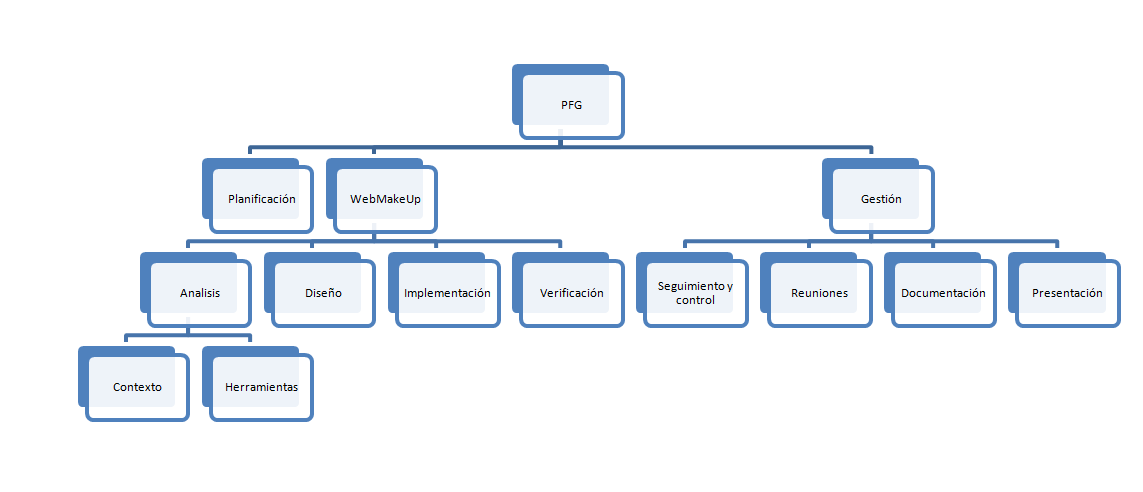
\includegraphics[width=0.95\textwidth]{figs/6-EDT.png}
\caption{Estructura de desglose de trabajo}
\label{fig:EDT}
\end{center}
\end{figure}

\begin{table}
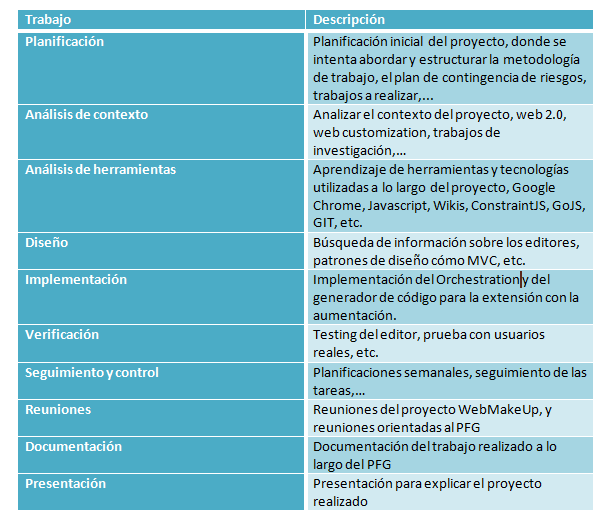
\includegraphics[width=0.95\textwidth]{figs/6-EDTTable.png}
\caption{Descripción de la estructura de trabajo.}
\label{tab:EDT}
\end{table}

\subsection{Diagrama de GANTT e Hitos}
\label{sec:GANTTEHitos}

Dada la naturaleza del proyecto es complejo definir en la línea temporal el cómo se va a desarrollar el proyecto, estimar tiempos o incluso delimitar las fases que hay a lo largo del mismo. Todo va a estar condicionado a medida que se van obteniendo ideas, que modifican continuamente, tanto los objetivos, cómo las herramientas a desarrollar.

Para demostrar la complejidad de definir un diagrama de Hitos, se han dado dos hechos que surgen a lo largo del PFG y que no se prevén en el momento de la planificación:
\begin{itemize}
\item{Durante el mes de enero se decide por parte del grupo de investigación Onekin enviar el proyecto WebMakeUp al congreso ICWE 2014 \footnote{Página web del sitio ICWE 2014: \url{http://icwe2014.webengineering.org/}}. Esto hizo que se tuviera que aumentar el número de horas trabajadas durante el mes de enero.}
\item{Al alumno le sale la oportunidad de hacer prácticas en empresa durante tres meses. Esto hizo que descendiera el número de horas trabajadas frente a las previstas durante los meses de marzo, abril y mayo.}
\end{itemize}

Teniendo en cuenta que pueden suceder cosas de este tipo, se decidió hacer una planificación inicial en base a un desarrollo por iteraciones. Se pretende hacer una primera iteración teniendo en cuenta que se disponía de más tiempo en el primer trimestre con un \emph{Hello World} funcional de la aplicación que se refina reunión tras reunión. Se preparan diferentes prototipos y se van aceptando o descartando los cambios que se van añadiendo a la herramienta. En la segunda iteración, más corta, tras probar la herramienta con usuarios finales, se siguen haciendo mejoras en caso de que fuesen necesarias.

Tal cómo se muestra en la figura \ref{fig:Gantt} se dividen por un lado las dos iteraciones, y también la parte más relacionada con el proyecto y la gestión del PFG. Al haber tantos condicionantes y tantas incógnitas, a pesar de crear una planificación general al inicio, la metodología que se adopta es la de planificaciones semanales y control exhaustivo. Con ello, se ve cómo se modifica el objetivo del proyecto que no está claramente definido desde el inicio.

El no tener un objetivo excesivamente definido, por el tipo de proyecto que es, permite ir adaptándolo a medida que se va haciendo el desarrollo, teniendo un mayor margen de maniobra sobre los objetivos adoptados al inicio. El mayor inconveniente, es que al no tener una planificación demasiado restrictiva, se puede dar el caso de que no se consiguiera el objetivo de concluir con el desarrollo completo.

De igual manera, el desarrollo ágil implica que el desarrollo no se divide en cuatro fases (análisis, diseño, implementación y testing) claramente diferenciadas en la línea temporal. Se va pasando por esas cuatro fases de manera continua. De ahí la razón de que en la Figura \ref{fig:Gantt} las fases del desarrollo se solapen durante toda la iteración.

\begin{figure}
\begin{center}
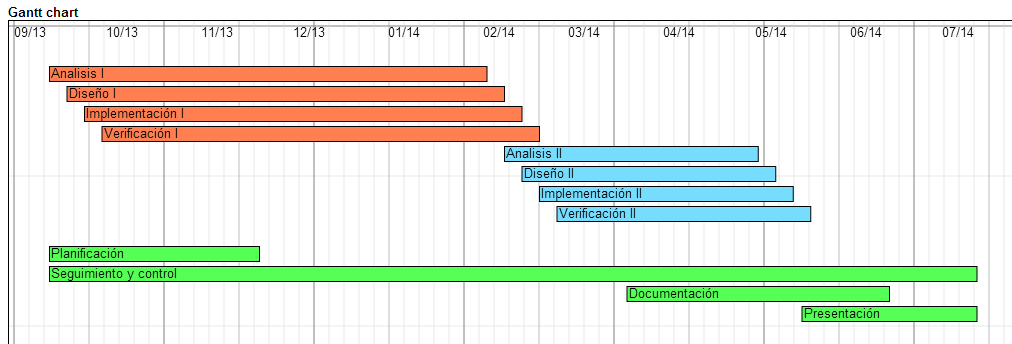
\includegraphics[width=0.65\textwidth]{figs/6-Gantt.png}
\caption{Diagrama de Gantt}
\label{fig:Gantt}
\end{center}
\end{figure}

\begin{figure}
\begin{center}
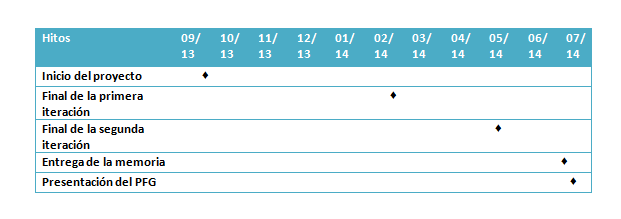
\includegraphics[width=0.65\textwidth]{figs/6-Hitos.png}
\caption{Diagrama de Hitos}
\label{fig:Hitos}
\end{center}
\end{figure}

Tal como se observa en el diagrama de la Figura \ref{fig:Hitos} existen cinco hitos que si se han definido desde un principio:

\begin{itemize}
\item{Comienzo del proyecto: 26 de septiembre de 2013. Fecha en la que se da inicio al proyecto y se pre-inscribe en GAUR.}
\item{Final de la primera iteración: finales de febrero.}
\item{Final de la segunda iteración: finales de abril.}
\item{Matriculación del proyecto en GAUR: 23 de junio de 2014 y a su vez entrega en ADDI del proyecto: 1 de julio de 2014 (fecha límite).}
\item{Final del proyecto: 16-18 de julio de 2014. Fecha en la que se presenta el proyecto ante el tribunal.}
\end{itemize}

En base a todas estas premisas, se hace una estimación de tiempo invertido en cada una de las fases del proyecto que se desglosa en la Tabla \ref{tab:TiemposPlanificacion}. Lógicamente esta tabla iba a ser simplemente orientativa, dado que los recursos de los que se dispone en este proyecto eran mayores. El uso de los recursos temporales principalmente depende de cómo se fuese desarrollando el proyecto y cómo se va disponiendo de ellos, dependiendo de la carga de las asignaturas del curso lectivo, que prevalecen en todo momento frente al PFG.

Como se observa en la Tabla \ref{tab:TiemposPlanificacion}, se hace una estimación donde se dedican algo más del 50\% al desarrollo del proyecto y el resto a planificación, seguimiento y documentación. La razón de ello es que al trabajar en grupo y al ser un proyecto de innovación es vital llevar un seguimiento muy exhaustivo. De igual manera, al trabajar con ideas innovadoras, hay que ser bastante meticuloso explicando lo que se ha desarrollado, ya que no es trivial, y por tanto dedicarle muchos recursos y aprovecharlos bien es importante. Por último, los valores añadidos que se quieren realizar con este proyecto requieren de trabajo en estos aspectos que no son puramente de desarrollo.

\begin{table}
\begin{center}
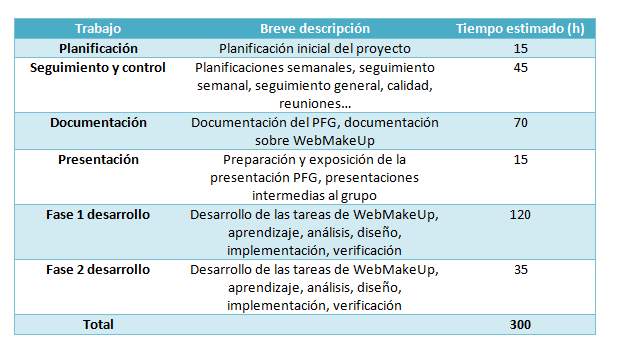
\includegraphics[width=0.95\textwidth]{figs/6-TiemposPlanificacion.png}
\caption{Tabla de tiempos planificados al inicio del proyecto}
\label{tab:TiemposPlanificacion}
\end{center}
\end{table}

\section{Metodología de trabajo}
\label{sec:MetodologiaTrabajo}

Cómo se describe en el Capítulo \ref{cha:Antecedentes} el PFG es una pequeña parte de lo que contiene el proyecto de WebMakeUp. Es conveniente explicar cuál es la metodología de trabajo con el resto de los integrantes (Apartado \ref{sec:TrabajoEnEquipo}), y la individual (Apartado \ref{sec:TrabajoIndividual}).

\subsection{Metodología de trabajo en equipo}
\label{sec:TrabajoEnEquipo}

Para describir la metodología de trabajo en equipo, primero hay que describir brevemente a los integrantes del grupo con sus roles correspondientes.

\begin{figure}
\begin{center}
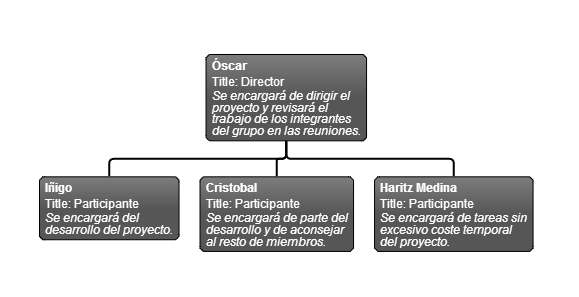
\includegraphics[width=0.95\textwidth]{figs/6-Equipo.png}
\end{center}
\caption{Organigrama del equipo de desarrollo de WebMakeUp}
\label{fig:OrganigramaEquipo}
\end{figure}

En la Figura \ref{fig:OrganigramaEquipo} se puede observar los integrantes del grupo con una breve descripción de su rol en el desarrollo de WebMakeUp. En la Tabla \ref{tab:Stakeholders} se puede observar todos los stakeholders del PFG.

\begin{table}
\begin{center}
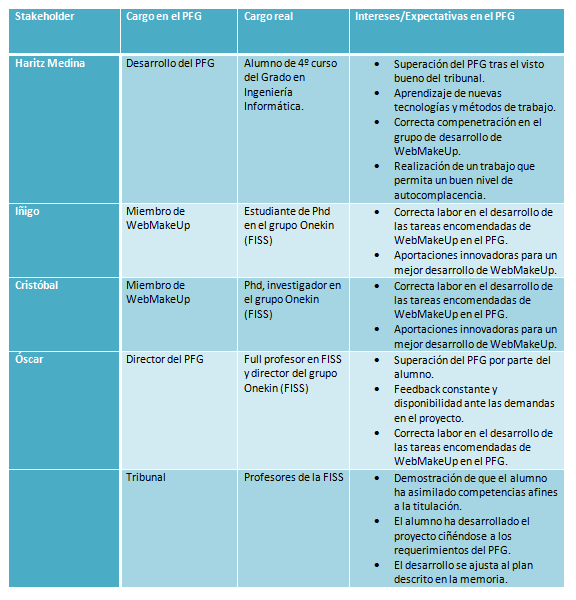
\includegraphics[width=0.95\textwidth]{figs/6-Stakeholders.png}
\end{center}
\caption{Tabla con los stakeholders del PFG}
\label{tab:Stakeholders}
\end{table}

Tras conocer esto, se utilizan diferentes herramientas para el trabajo en grupo. Para planificar las tareas y llevar un control de los deadlines \emph{Asana} (Anexo \ref{sec:Asana}). Para documentar \emph{Wiki de Onekin} (Anexo \ref{sec:Wiki}). Para el desarrollo un control de versiones de \emph{GIT en BitBucket} (Anexo \ref{sec:BitBucket}). Para intercambio de otros tipos de ficheros mediante correo y Dropbox (Anexo \ref{sec:Dropbox}).

Para las reuniones el alumno se encarga de alojar en la Wiki un topic con el acta por cada reunión. En esta se tienen en cuenta los siguientes aspectos:
\begin{itemize}
\item{Asistentes, duración, sitio (aunque casi siempre serán en el despacho de Óscar, director de proyecto).}
\item{Temas a tratar u orden del día (por parte de Óscar)}
\item{Presentación de trabajos realizados desde la anterior reunión.}
\item{Toma de decisiones.}
\item{Definición de tareas a realizar.}
\end{itemize}

Es importante asegurar que todos los presentes salen con trabajo a realizar para la próxima reunión y con las decisiones tomadas por escrito, para recordarlas.

Para el desarrollo de la aplicación, la comunicación ha de ser continua. Al trabajar sobre el mismo proyecto, se decide utilizar una plataforma de control de versiones como es GIT en este caso trabajando sobre la nube BitBucket para almacenamiento de las versiones.

Por último, para desarrollar las ideas en formato manuscrito se dispone de una Wiki. En ella se pueden hacer documentaciones de manera colaborativa y hablar de los diferentes aspectos de WebMakeUp.

\subsection{Metodología de trabajo individual}
\label{sec:TrabajoIndividual}

La metodología de trabajo individual consiste en diferentes aspectos entre los que se destacan los siguientes:
\begin{itemize}
\item{Planificación y realización de tareas: el sistema de planificación se ha basado en planificaciones continuas semanales. Además de utilizar la plataforma Asana, para un mejor desgranamiento de las tareas, se ha decidido utilizar una plataforma de gestión de tareas en Access (Anexo \ref{sec:Access}). En ella se deben de introducir las planificaciones semanales, se va realizando la gestión de las tareas y se ve el nivel de cumplimiento de las mismas. Al ser un proyecto complejo, el ir viendo que se alcanzan los objetivos a corto plazo es fundamental, no solo para poder asegurar el cumplimiento de un PFG de calidad, si no para garantizar el cumplimiento de los objetivos encomendados en el proyecto WebMakeUp, evitando desviarse en exceso en tareas no primordiales.}
\item{Seguimiento y control del PFG: a medida que se vaya desarrollando el PFG se verifican los objetivos a largo plazo. Esto se puede hacer en reuniones con el director y de manera individual. Aproximadamente se desarrollan reuniones con el director de manera mensual o bimensual para ir definiendo el objetivo y la forma del PFG.}
\item{Sistema de ficheros y de backups: una de las tareas más importantes es la de mantener la información de manera ordenada y actualizada, garantizando su persistencia frente a fallos de diferente índole. Los diferentes tipos de riesgos con pérdida de información están reflejados en la gestión de riesgos (Apartado \ref{sec:Riesgos}).

La información se distribuye en diferentes carpetas, tratando de mantener un orden estricto con tal de perder el menor tiempo posible en búsqueda de documentos. Se puede observar la estructura de ficheros de la Figura \ref{fig:EstructuraFicheros} entre los que destaca:
 \begin{itemize}
 \item{Bibliografía: documentos de lectura para aprendizaje e investigación.}
 \item{Compartido: ficheros de trabajo compartidos con otros integrantes del grupo. Destacan las carpetas sincronizadas con GIT.}
 \item{Documentación: documentación y agregados a la misma, cómo ejemplos, artículos de WebMakeUp enviados al congreso ICWE, etc.}
 \end{itemize}
 Las carpetas, para garantizar la disponibilidad en cualquier lugar, se almacenan en Dropbox. Esto a su vez ofrece un sistema de respaldo en nube y un control de versiones, que aunque sea muy básico, puede sacar de algún apuro. Para el código fuente (tanto el de WebMakeUp, cómo la memoria escrita en LaTeX) está también respaldado por un control de versiones. WebMakeUp en BitBucket, dado que tiene que ser un proyecto privado (no abierto al público). La memoria utiliza Google Code (Apartado \ref{sec:GoogleCode}). Por último, se hacen backups manuales periódicamente en otro disco duro externo para no tener que depender de las diferentes tecnologías en nube utilizadas.}
\item{Documentación: aunque esté planificada para final del PFG, es recomendable ir escribiendo algunos de los apartados a medida que se van completando, especialmente en el desarrollo y planificación. Estos se pueden documentar en la Wiki y en la fase de documentación hacer una migración a \LaTeX.}
\end{itemize}

\begin{figure}
\begin{center}
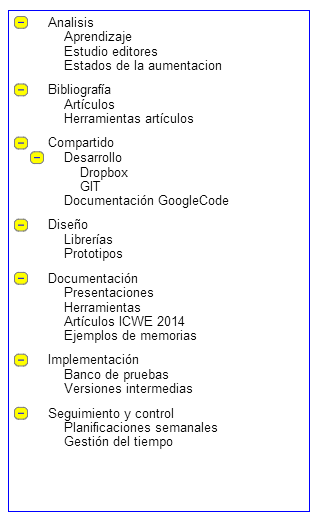
\includegraphics[width=0.35\textwidth]{figs/6-EstructuraFicheros.png}
\end{center}
\caption{Sistema de información general del PFG}
\label{fig:EstructuraFicheros}
\end{figure}

\section{Calidad}
\label{sec:Calidad}

Para definir el plan de calidad, hay que hablar de diferentes aspectos de la calidad. Por un lado la calidad del proyecto y por otro lado la calidad del producto que se quiere obtener. De igual manera, y haciendo una mención especial, también es interesante la calidad de los conocimientos adquiridos, especialmente en un proyecto innovador de investigación que se aborda por primera vez para el alumno. Por tanto se subdivide el plan de calidad abordando estos tres ámbitos:

\subsection{Orientado al PFG}
En referencia al Proyecto Final de Grado se quieren obtener estos niveles de calidad:
\begin{itemize}
\item{Una planificación lo más afín y realista posible. A medida que se vaya realizando planificaciones semanales se han de estimar de mejor manera tanto las tareas cómo su duración. Métrica que se define es la de contabilizar el número de tareas aplazadas. Para ello se crearán estadísticas con el gestor de tareas (Apartado \ref{sec:Access}).}
\item{Documentación correctamente redactada. La métrica que se ha decidido definir es la de nº de lectores de la memoria que han conseguido comprender parte de la misma. Para ello se le ofrece la lectura de este documento a varias personas, para que puedan valorar que está correctamente redactada y que los términos son fácilmente comprensibles.}
\end{itemize}

\subsection{Orientado al desarrollo de WebMakeUp}

El siguiente apartado se centra en explicar las métricas asociadas al desarrollo de WebMakeUp. Qué métricas definir para garantizar un desarrollo sencillo, útil, fácilmente legible, etc.

\begin{itemize}
\item{Código fuente correctamente documentado: para ello se define la métrica de cuantas funciones están correctamente documentadas. Si pueden estar definidas en JSDoc\footnote{JSDoc trata de emular a JavaDoc pero para aplicaciones en javascript: \url{http://usejsdoc.org/}}, mejor.}
\item{Código fuente sencillo: para ello se ha definido la métrica de cuantas líneas de media tiene cada función javascript del código programado.}
\item{Código fuente que permita un desarrollo más ágil: la métrica utilizada es cuántas de las clases o partes del código programado siguen un patrón de diseño (observer, singleton, facade,...) o una arquitectura adecuada (ya sea MVC, MV, arquitectura en 3 niveles, etc.)}
\item{Cumplimiento con estándares de ECMAScript 5. La métrica utilizada es en el código javascript cuantas funciones inician con \emph{``use strict``;}. Esto se encarga de evitar ciertos tipos de errores. En la Figura \ref{fig:UseStrict}} se puede observar una función con el preámbulo \emph{``use strict``;}.
\item{Programación orientada a seguir un proceso igual en todos las funciones. Para ello el editor utilizado, WebStorm\footnote{Sitio web de JetBrains/WebStorm: \url{http://www.jetbrains.com/webstorm}}, dispone de un corrector de código que detecta malos hábitos de programación. En este caso las métricas son cuantas variables se inicializan y cuantas no (dado que en Javascript no es obligatorio inicializarlas, pero si recomendable). Además también se define la métrica de bloques correctamente definidos (apertura y cierre de \emph{if}, \emph{whiles}, \emph{for} etc. con llaves \{\}, dado que en Javascript los bloques de una línea no lo requieren, pero es una buena práctica).}
\end{itemize}

\begin{figure}
\begin{center}
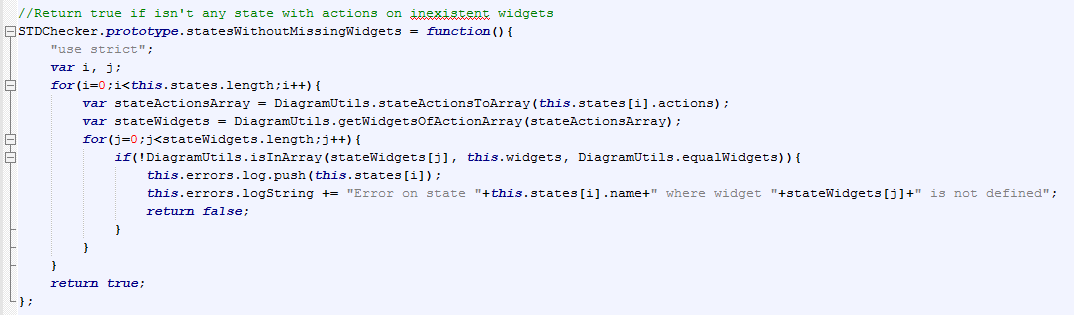
\includegraphics[width=0.95\textwidth]{figs/6-UseStrict.png}
\end{center}
\caption{Función javascript que cumple con el estandar ECMAScript 5}
\label{fig:UseStrict}
\end{figure}

\subsection{Orientado a la adquisición de conocimientos}

En este último apartado de calidad, se trata de valorar la calidad de los conocimientos adquiridos. Para ello se definen dos métricas:

\begin{itemize}
\item{Aplicabilidad de los conocimientos adquiridos: Número de artículos leídos donde se comprenda su contexto, significado y se pueda utilizar en el proyecto.}
\item{Aprendizaje autónomo sobre herramientas y tecnologías no utilizadas previamente. La métrica utilizada es la de búsqueda de mejora de técnicas de trabajo y su aplicación con éxito dentro del proyecto. Algunos ejemplos pueden ser: uso de control de versiones, uso tecnologías de documentación como Wikis, \LaTeX{},...}
\end{itemize}

Tras la realización del proyecto, los resultados de estas métricas están definidas en el Apartado \ref{sec:Resultados}.


\section{Riesgos}
\label{sec:Riesgos}

En un proyecto de estas características tener un plan de identificación y mitigación de riesgos es bastante importante, dado que el objetivo es a largo plazo. Además al ser un proyecto tan incierto el nivel de incógnita aumenta y los riesgos son más impredecibles.

En la Tabla \ref{tab:Riesgos} se refleja algunos de los riesgos que se han identificado, qué probabilidad existe de que ocurra, qué impacto tendría en el desarrollo del PFG, cómo prevenirlo y qué se podría hacer en caso de que ocurra.

\begin{table}
\begin{center}
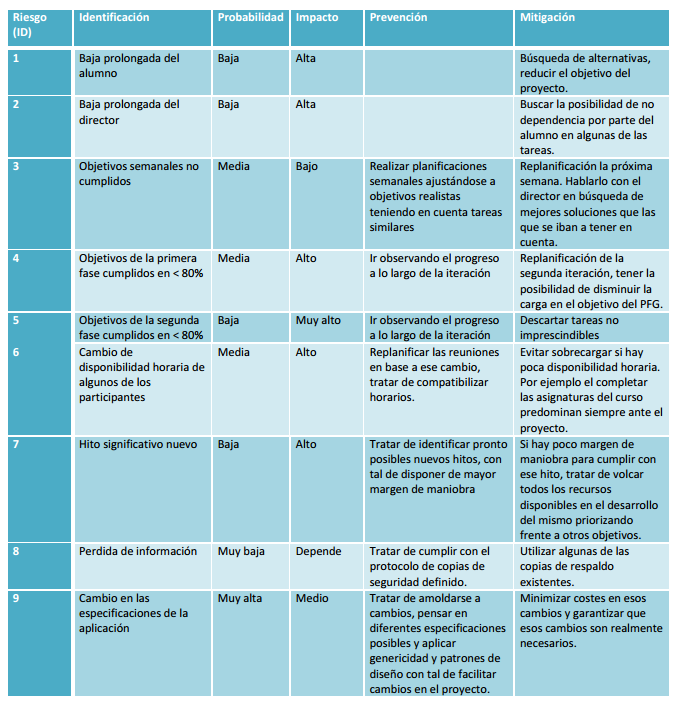
\includegraphics[width=0.95\textwidth]{figs/6-Riesgos.png}
\end{center}
\caption{Identificación y mitigación de riesgos}
\label{tab:Riesgos}
\end{table}


\section{Seguimiento y control}
\label{sec:Seguimiento}

En este apartado se comentan los aspectos de seguimiento y control más relevantes. Entre ellos, destacan los aspectos de gestión de tareas, replanificaciones, gestión de riesgos y trabajo en equipo.

En lo que a \textbf{gestión de tareas} se refiere cabe destacar que de lo planificado, a lo finalmente realizado, hay ciertos desajustes. En primer lugar cabe destacar que en la planificación se distribuyen en diferentes tipos de tareas y hay cambios. En la Tabla \ref{tab:RedistribucionTareas} se muestra los tipos de tareas que se planifican al principio del proyecto (Apartado \ref{sec:EDT}), y cómo han variado según las necesidades que surgen a lo largo del proyecto.

\begin{table}
\begin{center}
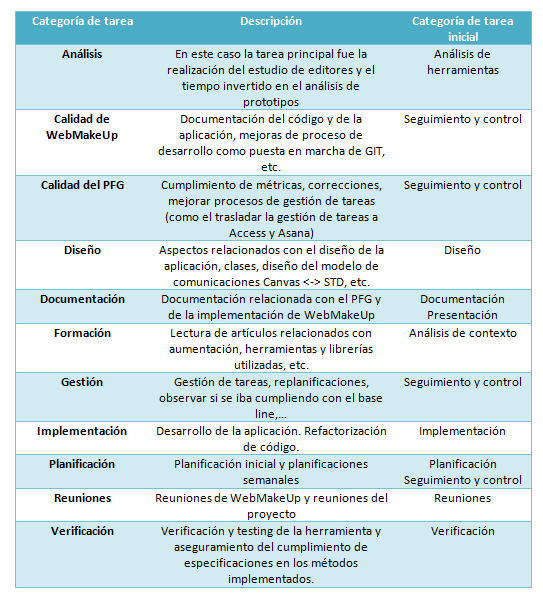
\includegraphics[width=0.95\textwidth]{figs/6-RedistribucionTareas.png}
\end{center}
\caption{Tabla comparativa de categorías de tareas planificadas en un inicio y utilizadas finalmente.}
\label{tab:RedistribucionTareas}
\end{table}

Junto con estos cambios, las \textbf{re-planificaciones} que se desarrollan son por diferentes causas. En un primer momento los hitos definidos son cinco, tal y como se comenta en el Apartado \ref{sec:GANTTEHitos}. Aún así a lo largo del proyecto surgen nuevos Hitos y cambios con respecto a la planificación.

En este caso se destacan principalmente dos hechos que cambian en gran parte la planificación inicial del proyecto.

\subsection{Re-planificación en base al congreso ICWE 2014}
Esta re-planificación surge después de que en el grupo Onekin decide presentar WebMakeUp al congreso ICWE 2014 que se celebra en Toulouse del 1 al 4 de Julio. El congreso ICWE es un congreso internacional donde participan ingenieros con tal de poder compartir ideas innovadoras y conceptos basados en software sobre sistemas web.

Para poder presentarse al congreso hay que presentar un \emph{paper}. Este no se realiza en el PFG. Un \emph{paper} es un artículo que comenta por un lado una idea innovadora y a su vez una pequeña explicación de un desarrollo concreto sobre esa idea. Por tanto, es necesario tener al menos una primera versión funcional de WebMakeUp para poder dar la explicación sobre el desarrollo.

A inicios de enero se fija este nuevo hito, que es para el día 18 de febrero. Esto requiere de un mayor esfuerzo y dedicación durante el mes de enero y especialmente a medida que se aproxima la fecha del hito. Es importante trabajar de manera coordinada y a su vez disponer de tiempo para la realización del mismo. El mes de enero por parte del alumno es en el que más tiempo se dispone. Por tanto, se puede dedicar enteramente al desarrollo de WebMakeUp. Asimismo, se fijan reuniones con mayor frecuencia, incluso diarias durante la última semana, dado el momento crítico en el que se encuentra el proyecto para cumplir con este hito. Tal y cómo se puede observar en la Figura \ref{fig:graficoReuniones}, la carga de comunicación (tiempo dedicado a reuniones) es mucho mayor en las semanas próximas a febrero que en el resto del PFG.

\begin{figure}
\begin{center}
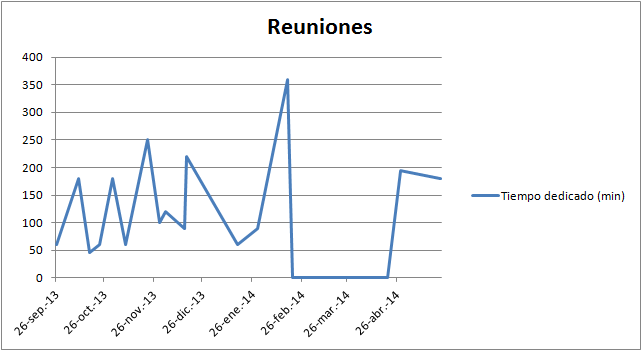
\includegraphics[width=0.65\textwidth]{figs/6-GraficoReuniones.png}
\end{center}
\caption{Tiempo (en minutos) invertido en reuniones a lo largo del PFG.}
\label{fig:graficoReuniones}
\end{figure}

\subsection{Re-planificación en base a realización de prácticas en empresa}

Otra de las claves en lo que a re-planificación se refiere es la realización de prácticas en empresa por parte del alumno. Estas se realizan entre mediados de febrero y mediados de mayo. Consisten en una dedicación de 20 horas semanales (media jornada) y se compaginan con las 2 asignaturas que se estaban cursando en el segundo cuatrimestre. La realización de estas prácticas y las asignaturas no permiten dedicar tiempo al PFG.

Las razones de la realización de las prácticas se deben a diferentes causas:
\begin{itemize}
\item{Propósito de obtener experiencia en el mundo laboral. Estas prácticas no son necesarias para el cumplimiento de los créditos del curso académico.}
\item{El trabajo realizado en el PFG sobrepasa las expectativas para aquella fecha. En gran parte esto es debido a la inversión de tiempo extra realizado para el congreso ICWE.}
\item{Dado que el desarrollo de WebMakeUp en esas fechas requiere de refactorización del código y prueba con usuarios finales que no está incluida en este PFG, no se requiere de mayor labor hasta conocer ese \emph{feedback} por parte de usuarios finales.}
\end{itemize}

Posteriormente, al finalizar las prácticas se vuelve a retomar haciendo una pequeña segunda iteración del proyecto. En él, atendiendo al feedback de los usuarios, se traslada el generador de extensiones de WebMakeUp al modelo basado en blinks explicado en el Apartado \ref{sec:modeloBlinks}.

La \textbf{gestión de riesgos} consigue solventar gran parte de los problemas. Cabe destacar que el tiempo extra dedicado en la primera fase del proyecto, hasta el hito de ICWE, consigue solventar con seguridad los objetivos para la primera iteración. Pero no sólo eso, si no que se realiza un proyecto para aquellas fechas que ya cubre lo que se esperaba realizar en la segunda iteración y por tanto a lo que se espera que fuese el desarrollo del PFG en si.

La prevención juega un papel fundamental. Por ejemplo, en poder lograr cumplir con el hito de la conferencia ICWE. Además, la rápida detección de la posibilidad de prácticas en empresa (ya se conoce desde principios de Enero), se puede establecer una planificación acorde a la situación. En ella se trabaja más en enero, mayo y junio permitiendo cumplir con todos los hitos restantes del PFG.

Aún así, en la Tabla \ref{tab:RiesgosNoPlanificados} se observan algunos de los riesgos que no se tuvieron en cuenta en la planificación. Se muestran los riesgos, el impacto y cómo se solventan.

\begin{table}
\begin{center}
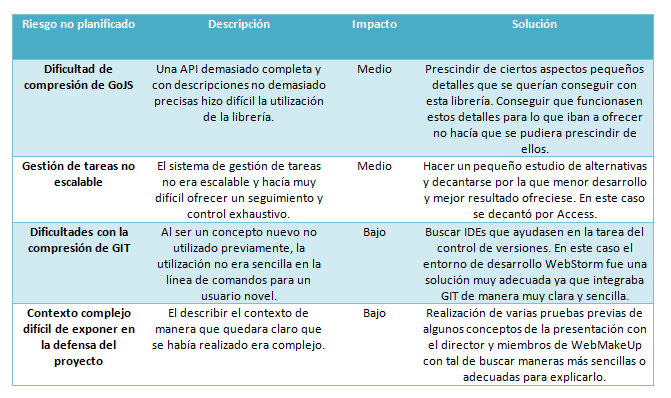
\includegraphics[width=0.95\textwidth]{figs/6-RiesgosNoPlanificados.png}
\end{center}
\caption{Otros riesgos que han surgido a lo largo del proyecto y no estaban planificados.}
\label{tab:RiesgosNoPlanificados}
\end{table}

Cómo se observa, son riesgos sin demasiado impacto y solventados sin excesivo problema o coste. En parte esto se debe a la buena planificación de riesgos realizada, bastante pesimista y teniendo en cuenta los peores casos con tal de garantizar la finalización con mayor probabilidad. También, influye la cantidad de recursos de tiempo de la que se dispone a lo largo del curso, que es grande. Esto facilita mucho la labor, pudiendo anticipar la realización de muchas de las tareas.

Por último, teniendo en cuenta los aspectos de seguimiento, el \textbf{desarrollo en equipo} ha ido de manera correcta. Las reuniones en grupo han sido muy útiles y se han seguido los aspectos fundamentales que se definieron al inicio del PFG. En el Anexo \ref{sec:ActasDeReunion} se puede observar un acta de reunión donde se verifican algunos de estos aspectos.

\section{Resultados}
\label{sec:Resultados}

En este apartado se trabajan principalmente dos aspectos. Por un lado, el grado de cumplimiento con los plazos y estimaciones establecidos. Por otro lado, el grado de calidad con el que se ha hecho en base a las métricas planificadas.

Antes de comenzar con el \textbf{grado de cumplimiento de plazos y estimaciones}, un apunte. Las estadísticas aquí reflejadas no contabilizan el total real de las horas dedicadas planificadas semanalmente o realizadas. La razón es que parte del desarrollo del PFG es describir esta misma memoria. Para contabilizar el total absoluto habría que hacerlo una vez acabada y verificada la memoria. Asimismo hay que añadir horas de preparación de la exposición del PFG, donde hay ciertas partes que se hacen después de la memoria. Por tanto, los datos aquí presentes son hasta el día 19 de junio de 2014. De igual manera, la contabilidad de estas horas representan más del 95\% del total, lo que es una mayoría suficiente con la que sacar conclusiones.

Para verificar en qué medida se desvían los resultados en base a la planificación inicial, hay que basarse en el tiempo planificado para cada apartado y el tiempo real dedicado. Para ello en el inicio se definen 300 horas de trabajo. Simplemente es un objetivo mínimo dado que los recursos temporales disponibles son mayores y depende del interés en el proyecto el tiempo que se dedica finalmente.

\begin{figure}
\begin{center}
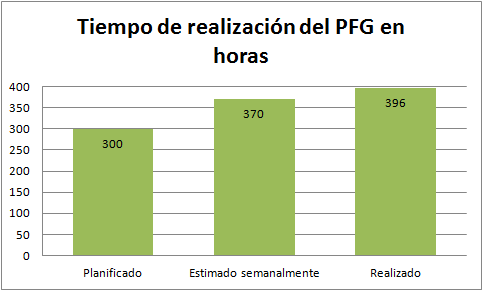
\includegraphics[width=0.40\textwidth]{figs/6-TiemposTotales.png}
\end{center}
\caption{Tiempo del PFG planificado, estimado de manera semanal y real.}
\label{fig:TiemposTotales}
\end{figure}

En la Figura \ref{fig:TiemposTotales} se muestran tres columnas. En la primera se observa el tiempo planificado inicialmente 300 horas. En la segunda en base a las planificaciones semanales cuánto se estimaba en total. En la tercera columna, el tiempo real dedicado al PFG. Este gráfico muestra cómo a medida que se conocen las tareas a realizar se aproximan las estimaciones a la realidad. En este tipo de proyectos con gran parte innovadora y orientada a la investigación, no tiene sentido realizar una planificación a largo plazo. En este gráfico se muestra que esto es así, dado que la planificación inicial difiere en más de un 15\% del tiempo dedicado finalmente.

En la Figura \ref{fig:TiemposPorCategoria} se pueden observar tres columnas por cada categoría. El glosario es idéntico al gráfico anterior, pero aquí se observa más claro en qué se han dedicado los esfuerzos, cual de las categorías de tareas se planifica mejor y en qué aspectos hay un menor control.

\begin{figure}
\begin{center}
\subfloat[Tiempo en minutos de las categorías]{
	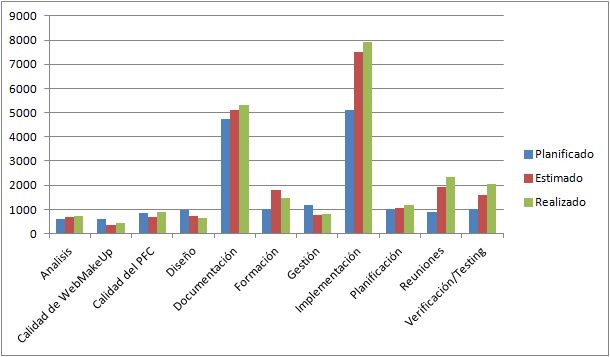
\includegraphics[width=0.45\textwidth]{figs/6-TiemposPorCategoria.png}
	
}
\subfloat[Tiempo en porcentaje respecto al total de las categorías]{
	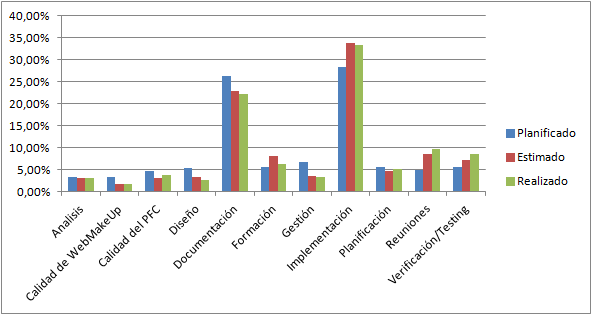
\includegraphics[width=0.50\textwidth]{figs/6-PorcentajesPorCategoria.png}
}
\end{center}
\caption{Tiempo (en minutos y porcentaje) de las categorías planificado (azul), estimado de manera semanal (rojo) y realizado (verde).}
\label{fig:TiemposPorCategoria}
\end{figure}

En este caso cabe destacar cómo la mayor diferencia se encuentra en la parte de implementación. En ella, la planificación es demasiado optimista, dado que se tarda casi 50 horas más de lo planificado inicialmente. 
Esto se debe en gran parte a dos factores. El tiempo dedicado en total en el PFG es mayor que el planificado, por tanto la estadística se podría decir que está un poco desvirtuada. Para ello, el segundo gráfico muestra con mayor precisión la planificación frente a lo realizado. El segundo factor está relacionado a lo que es la tónica en este tipo de proyectos, la mayor dificultad se encuentra en la parte menos elaborada o trillada, en este caso el desarrollo. En él se utilizan librerías con poca o ninguna documentación. El desarrollo es en equipo, lo que aumenta los problemas. Asimismo, y no menos importante, la poca dedicación al diseño y el desconocimiento del lenguaje nunca trabaja en favor de una implementación rápida. Por último, en la planificación se desconoce qué se desarrolla realmente, por tanto es poco probable ''acertar''. A pesar de ello, tampoco es ese el objetivo de la planificación, si no el definir unas pautas y metodologías a seguir.

Hablando de la \textbf{calidad del proyecto}, basándose en las métricas definidas en el Apartado \ref{sec:Calidad}, se observa en qué medida se consigue un PFG con la calidad inicialmente deseada. En las Tablas \ref{tab:Metricas} se muestra en base a las tres categorías definidas en la gestión de calidad, el grado de cumplimiento. Se define la métrica, cuál fue el nivel exigido al inicio del PFG y el grado de cumplimiento.

\begin{table}
\begin{center}
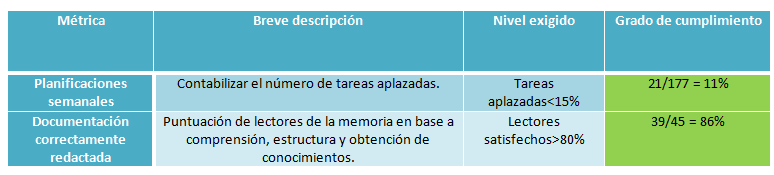
\includegraphics[width=0.95\textwidth]{figs/6-MetricasPFG.png}
Métricas relacionadas con la calidad del PFG.
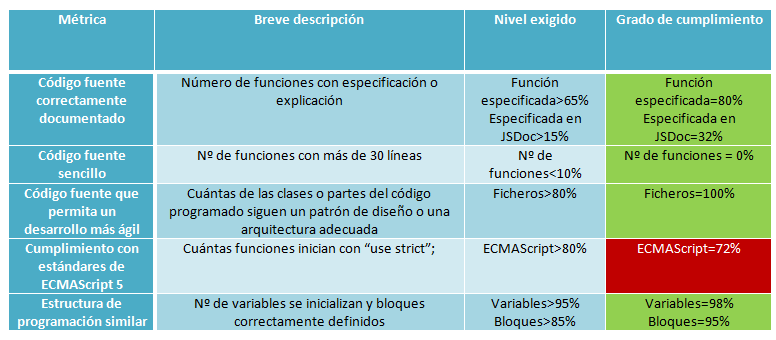
\includegraphics[width=0.95\textwidth]{figs/6-MetricasWebMakeUp.png}
Métricas relacionadas con la calidad del desarrollo de WebMakeUp.
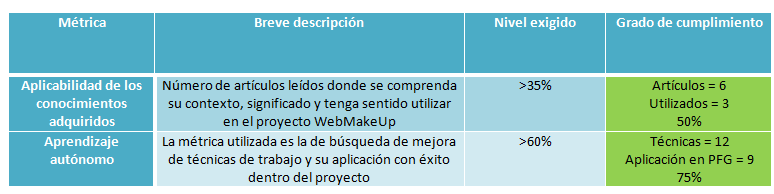
\includegraphics[width=0.95\textwidth]{figs/6-MetricasConocimientos.png}
Métricas relacionadas con la aplicabilidad de conocimientos adquiridos.
\end{center}
\caption{Métricas definidas en la gestión de calidad y su grado de cumplimiento en el desarrollo del PFG.}
\label{tab:Metricas}
\end{table}

Teniendo en cuenta estas métricas, se puede extraer de conclusión que el nivel exigido en el tema de calidad es muy útil para completarlo. A su vez sirve para establecer ciertos niveles de exigencia. A pesar de que no se cumplen todos los objetivos, los resultados obtenidos sirven para mejorar en futuras ocasiones. Principalmente, lo que cabe destacar, es que definir estos mínimos de calidad sirve para el aprendizaje personal. Con ello se ve cual es la dificultad de cumplir con exigencias en un proyecto de un volumen medianamente grande.
